% Paquets généraux
\documentclass[a4paper,12pt,titlepage,twoside]{article}
\usepackage[T1]{fontenc}
\usepackage[utf8]{inputenc}
\usepackage[french]{babel}
\usepackage[gen]{eurosym}
%\usepackage[dvips]{graphicx}
\usepackage{fancyhdr}
\usepackage{pdfpages} 
\usepackage{multido}
\usepackage{enumitem}
\usepackage{hyperref}
%\usepackage{textcomp}
%\usepackage{aeguill}
\usepackage{schemabloc}
\usepackage[bitstream-charter]{mathdesign}

\newcommand{\id}{71}
\newcommand{\nom}{Théorie des mécanismes}
\newcommand{\sequence}{04}
\newcommand{\nomsequence}{Liaisons entre les solides}
\newcommand{\num}{02}
\newcommand{\type}{KH}
\newcommand{\descrip}{Liaisons équivalentes, hyperstatisme, liaisons en série et en parallèle, théorie des graphes}
\newcommand{\competences}{B2-12: Proposer une modélisation des liaisons avec leurs caractéristiques géométriques. \\ &  B2-13: Proposer un modèle cinématique paramétré à partir d'un système réel, d'une maquette numérique ou d'u \\ &  B2-17: Simplifier un modèle de mécanisme. \\ &  B2-18: Modifier un modèle pour le rendre isostatique. \\ &  C1-04: Proposer une démarche permettant d'obtenir une loi entrée-sortie géométrique.  \\ &  C2-05: Caractériser le mouvement d'un repère par rapport à un autre repère. \\ &  C2-06: Déterminer les relations entre les grandeurs géométriques ou cinématiques. }
\newcommand{\nbcomp}{7}
\newcommand{\systemes}{}
\newcommand{\systemesnum}{}
\newcommand{\systemessansaccent}{}
\newcommand{\ilot}{2}
\newcommand{\ilotstr}{02}
\newcommand{\dossierilot}{\detokenize{Ilot_02 }}


\newcommand{\institute}{Lycée Dorian}

\renewcommand{\epsilon}{\varepsilon}

\usepackage{color}
\usepackage{xcolor}
\usepackage{colortbl}
\usepackage{helvet}
\renewcommand{\familydefault}{\sfdefault}
\usepackage[frenchmath]{newtxsf} % for sans serif symbols
%\usepackage{amsfonts}
%\usepackage{amsmath}
%\usepackage{xspace}
\usepackage{varioref}
\usepackage{tabularx}
%\usepackage{floatflt}
\usepackage{graphics}
\usepackage{wrapfig}
\usepackage{textcomp}
\usepackage{tikz}
\usepackage{wrapfig}
\usepackage{gensymb}
\usepackage[european]{circuitikz}
\usetikzlibrary{babel}
\usepackage{ifthen}
\usepackage{cancel}
\usepackage{etoolbox}
\usepackage{multirow}
%\usepackage{boxedminipage}
\definecolor{gris25}{gray}{0.75}
\definecolor{bleu}{RGB}{18,33,98}
\definecolor{bleuf}{RGB}{42,94,171}
\definecolor{bleuc}{RGB}{231,239,247}
\definecolor{rougef}{RGB}{185,18,27}
\definecolor{rougec}{RGB}{255,188,204}%255,230,231
\definecolor{vertf}{RGB}{103,126,82}
\definecolor{vertc}{RGB}{220,255,191}
\definecolor{forestgreen}{rgb}{0.13,0.54,0.13}
\definecolor{blcr}{rgb}{0.59,0.69,0.84}
\definecolor{blfr}{rgb}{0.32,0.51,0.75}
\definecolor{orfr}{rgb}{0.90,0.42,0.15}
\definecolor{orcr}{rgb}{0.90,0.65,0.50}
\definecolor{orangef}{rgb}{0.659,0.269,0.072}
\definecolor{orange}{rgb}{0.58,0.35,0.063}
\definecolor{orangec}{rgb}{0.43,0.32,0.25}
\definecolor{rcorrect}{rgb}{0.6,0,0}
\definecolor{sequence}{rgb}{0.75,0.75,0.75}
\definecolor{competences}{rgb}{0.61,0.73,0.35}
\definecolor{grisf}{HTML}{222222}
\definecolor{grisc}{HTML}{636363}
\definecolor{normal}{HTML}{4087c4}
\definecolor{info}{HTML}{5bc0de}
\definecolor{success}{RGB}{92,184,92}
\definecolor{warning}{RGB}{240,173,78}
\definecolor{danger}{RGB}{217,83,79}
\hypersetup{                    % parametrage des hyperliens
    colorlinks=true,                % colorise les liens
    breaklinks=true,                % permet les retours à la ligne pour les liens trop longs
    urlcolor= blfr,                 % couleur des hyperliens
    linkcolor= orange,                % couleur des liens internes aux documents (index, figures, tableaux, equations,...)
    citecolor= forestgreen                % couleur des liens vers les references bibliographiques
    }

% Mise en page
%\pagestyle{fancy}

\setlength{\hoffset}{-18pt}

\setlength{\oddsidemargin}{0pt} 	% Marge gauche sur pages impaire2s
\setlength{\evensidemargin}{0pt} 	% Marge gauche sur pages paires
\setlength{\marginparwidth}{00pt} 	% Largeur de note dans la marge
\setlength{\headwidth}{481pt} 	 	% Largeur de la zone de tête (17cm)
\setlength{\textwidth}{481pt} 	 	% Largeu\textbf{r de la zone de texte (17cm)
\setlength{\voffset}{-18pt} 		% Bon pour DOS
\setlength{\marginparsep}{7pt}	 	% Séparation de la marge
\setlength{\topmargin}{-30pt} 		% Pas de marge en haut
\setlength{\headheight}{35pt} 		% Haut de page
\setlength{\headsep}{20pt} 		% Entre le haut de page et le texte
\setlength{\footskip}{30pt} 		% Bas de\textbf{ page + séparation
\setlength{\textheight}{700pt} 		% Hauteur de l'icone zone de texte (25cm)
\setlength\fboxrule{1 pt}
\renewcommand{\baselinestretch}{1}
\setcounter{tocdepth}{1}
\newcommand{\cadre}[2]
{\fbox{
  \begin{minipage}{#1\linewidth}
   \begin{center}
    #2\\
   \end{center}
  \end{minipage}
 }
}

\newcounter{num_quest} \setcounter{num_quest}{0}
\newcounter{num_rep} \setcounter{num_rep}{0}
\newcounter{num_cor} \setcounter{num_cor}{0}

\newcommand{\question}[1]{\refstepcounter{num_quest}\par
~\ \\ \textbf{Question \arabic{num_quest} : }#1\label{q\the\value{num_quest}}\par
}


\newcommand{\feuilleDR}[1]{
	\begin{tikzpicture}
		\draw[gray!30](0,0)grid[step=0.5cm](\linewidth,#1);
	\end{tikzpicture}
}


\newcommand{\reponse}[4][1]
{\noindent
\parbox{\textwidth}{
\rule{\linewidth}{.5pt}\\
\textbf{Question\ifthenelse{#1>1}{s}{} \multido{}{#1}{%
\refstepcounter{num_rep}\ref{q\the\value{num_rep}} }:} ~\ \\
\ifdef{\public}{#3 \ifthenelse{#2>0}{~\ \\ 	\feuilleDR{#2}}}{#4}
}}

\newcommand{\cor}
{\refstepcounter{num_cor}
\noindent
\rule{\linewidth}{.5pt}
\textbf{Question \arabic{num_cor}:} \\
}

\newcommand{\titre}[1]
{\begin{center}
\cadre{0.8}{\huge #1} 
\end{center}
}

\makeatletter
\newcommand\modulo[2]{
    \newcounter{lastpagesujet}
	\setcounter{lastpagesujet}{#1}
    \divide\value{lastpagesujet} by #2
    \multiply\value{lastpagesujet} by #2\relax
    }
\makeatother

\newcommand{\finsujet}[1]
{
    \begin{center}
    \Large{FIN}
    \end{center}
    
    \ifthenelse{\equal{#1}{public}}{\def\public{}}{}

	\newpage
	
    \ifdef{\public}{
    	\modulo{\value{page}}{2}
		\whiledo{\value{page}<\value{lastpagesujet}}{~\ \newpage}
        \pagestyle{docreponse}
	}{\pagestyle{correction}}

    \ifdef{\public}{
        \begin{tikzpicture} 
            \draw (0,0) rectangle (2,2);
            \draw (0,0) -- (2,2);
            \draw (1.5,0.5) node {\large 20};
            \draw (2.5,0) rectangle (16,2);
            \draw (4.5,1.7) node {\large Commentaires:};
        \end{tikzpicture}
    }
    ~\ \\
}

% En tête et pied de page
\fancypagestyle{normal}{%
\fancyhf{}
\lhead{\sujet\ -\ NOM Prénom: .............................}
\rhead{
\includegraphics[width=2cm]{../../../img/logo}\hspace{2pt}}
\ifdef{\auteurdeux}{\lfoot{\auteurun,\ \auteurdeux}}{\lfoot{\auteurun}}
\rfoot{\nom}
}

\fancypagestyle{docreponse}{%
\fancyhf{}
\fancyhead[LO]{NOM Prénom: .............................}
\rhead{
\includegraphics[width=2cm]{../../../img/logo}\hspace{2pt}}
\ifdef{\auteurdeux}{\lfoot{\auteurun,\ \auteurdeux}}{\lfoot{\auteurun}}
\rfoot{\nom}
}

\fancypagestyle{correction}{%
  \fancyhf{}
  \lhead{\colorbox{danger}{\begin{minipage}{0.65\paperwidth} \textcolor{white}{\textbf{Correction}} \end{minipage}} }
  \rhead{
\includegraphics[width=2cm]{../../../img/logo}}
  \ifdef{\auteurdeux}{\lfoot{\auteurun,\auteurdeux}}{\lfoot{\auteurun}}
  \rfoot{\colorbox{danger}{\begin{minipage}{0.5\paperwidth} \begin{flushright}\textcolor{white}{\textbf{Correction}}\end{flushright} \end{minipage}} }}

\renewcommand{\footrulewidth}{0.4pt}

\usepackage{eso-pic}
\newcommand{\BackgroundPic}{%
\put(0,0){%
\parbox[b][\paperheight]{\paperwidth}{%
\vfill
\begin{center}
\hspace{0.5cm}\vspace{0.5cm}

\includegraphics[width=\paperwidth,height=\paperheight,%
keepaspectratio]{../../../img/fond3}%
\end{center}
\vfill
}}}

\newcommand{\BackgroundPicdeux}{%
\put(25,-30){%
\parbox[b][\paperheight]{\paperwidth}{%
\vfill
\begin{center}
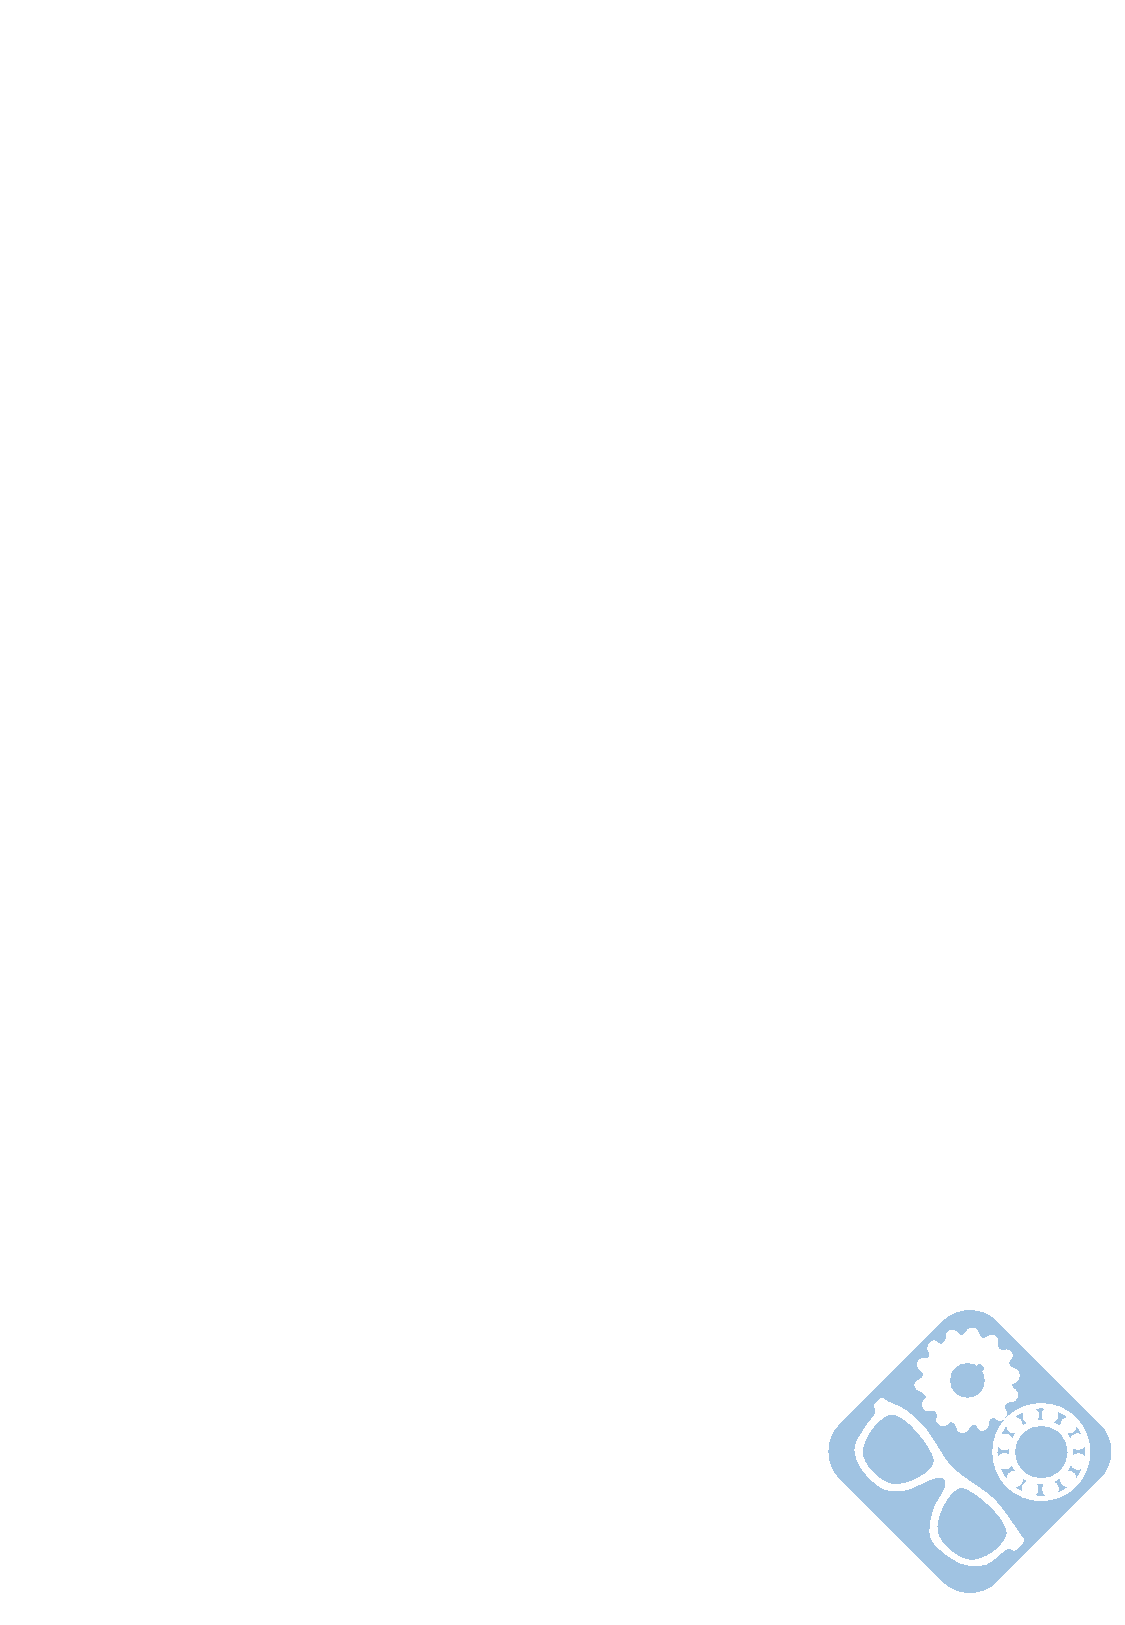
\includegraphics[width=\paperwidth,height=\paperheight,%
keepaspectratio]{../../../img/fond4}%
\end{center}
\vfill
}}}

\begin{document}

\AddToShipoutPicture{\BackgroundPicdeux}

\pagestyle{normal}


\section{Présentation}

\begin{figure}[!h]
  \begin{minipage}{0.35\linewidth}
  \centering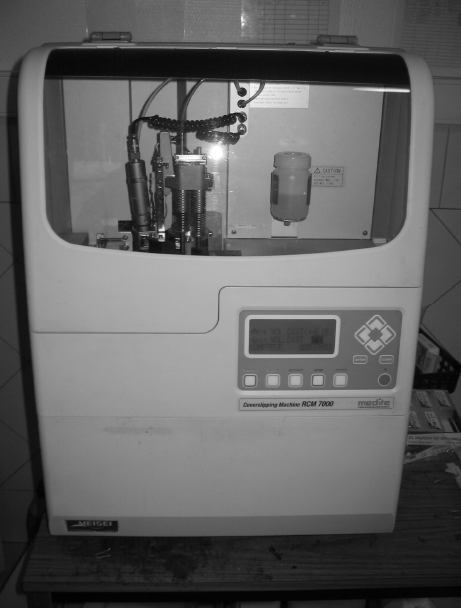
\includegraphics[width=0.8\linewidth]{img/colleuse.png}
  \caption{Colleuse}
  \label{img1}
  \end{minipage}
  \hfill
  \begin{minipage}{0.60\linewidth}
  Le groupe TECH-INTER commercialise du matériel de laboratoire d'histopathologie. Cette spécialité médicale consiste à découper des tissus d'organes en fine épaisseur ($4-5 \mu m$). Ces tissus sont ensuite collés sur des lames de verres de 2 mm d'épaisseur puis colorés chimiquement dans un automate. Pour certains tissus, il est nécessaire de coller sur les tissus colorés une lamelle de verre de 0,3 mm d'épaisseur afin de les protéger. Cette dernière opération est très délicate à effectuer manuellement et très longue, une étude pouvant comporter plusieurs centaines de lames.

  L'appareil appelé « Colleuse de lamelle » automatise ce procédé, figure \ref{img1}.
\end{minipage}
\end{figure}

\section{Analyse cinématique de l'élévateur de rack}

Le schéma cinématique, figure \ref{img2} représente le système d'élévateur de rack. Un moteur non représenté génère le mouvement d'entrée, soit la rotation de l'axe \textbf{10} par rapport à 0. Celui-ci entraîne, par un système vis-écrou comportant un pas à droite, le support de rack \textbf{11}. Les liaisons sont supposées parfaites. On fera la distinction entre les liaisons $\left\{V^B_{11/0}\right\}$ et $\left\{V^C_{11/0}\right\}$, entre les pièces 11 et 0, respectivement d'axes (B,$\vec{y_0}$) et (C,$\vec{y_0}$).

\question{A partir du schéma cinématique de la figure \ref{img2}, établir le graphe de liaison du mécanisme.}

\question{Écrire le torseur cinématique de chaque liaison.}

~\

Remarque : Ne pas oublier l'équation supplémentaire pour la liaison hélicoïdale, faisant intervenir le pas $p$ du filetage.

\question{Écrire les torseurs cinématiques $\left\{V^B_{11/0}\right\}$ et $\left\{V^C_{11/0}\right\}$ au point O.}

\question{Ecrire les 12 équations qui lient les composantes de ces liaisons et les paramètres géométrique du mécanisme.}

\newpage

\begin{figure}[!h]
  \centering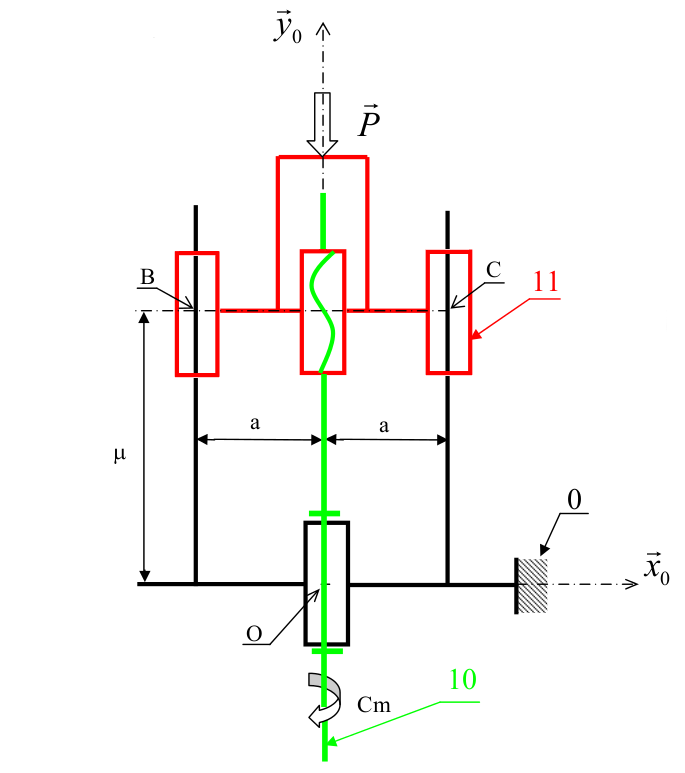
\includegraphics[width=0.6\linewidth]{img/colleuse_cin.png}
  \caption{Schéma cinématique}
  \label{img2}
\end{figure}

Rappels:

On notera le torseur cinématique du solide i par rapport au solide j exprimé au point M par :

\begin{center}
\begin{math}
\left\{V_{i/j}\right\}=\left\{
\begin{array}{cc}
\omega_{x,ij} & V_{x,M,ij} \\
\omega_{y,ij} & V_{y,M,ij} \\
\omega_{z,ij} & V_{z,M,ij}
\end{array}
\right\}_{X,R_P}
\end{math}, avec $R_P=(\overrightarrow{X_P},\overrightarrow{Y_P},\overrightarrow{Z_P})$
\end{center}

~\

\finsujet

\reponse{6}{}{
\begin{center}
\def\svgwidth{.6\linewidth}
\input{img/graphe_liaison.pdf_tex}
\end{center}
}

\reponse{12}{}{
$\left\{V_{1/0}\right\}=\left\{
\begin{array}{cc}
0 & 0 \\
\omega_{10} & 0 \\
0 & 0
\end{array}
\right\}_{O,R_0}$
$\left\{V^B_{11/0}\right\}=\left\{
\begin{array}{cc}
0 & 0 \\
\omega_{11B} & V_{11B} \\
0 & 0
\end{array}
\right\}_{B,R_0}$
$\left\{V^C_{11/0}\right\}=\left\{
\begin{array}{cc}
0 & 0 \\
\omega_{11C} & V_{11C} \\
0 & 0
\end{array}
\right\}_{C,R_0}$
$\left\{V_{11/10}\right\}=\left\{
\begin{array}{cc}
0 & 0 \\
\omega_{1110} & V_{1110} \\
0 & 0
\end{array}
\right\}_{O,R_0}$, avec $V_{1110}=\dfrac{p}{2\cdot\pi}\cdot\omega_{1110}$.
}


\reponse{10}{}{
$\left\{V^B_{11/0}\right\}=\left\{
\begin{array}{cc}
0 & 0 \\
\omega_{11B} & V_{11B} \\
0 & -a\cdot \omega_{11B}
\end{array}
\right\}_{O,R_0}$
$\left\{V^C_{11/0}\right\}=\left\{
\begin{array}{cc}
0 & 0 \\
\omega_{11C} & V_{11C} \\
0 & a\cdot \omega_{11C}
\end{array}
\right\}_{O,R_0}$

}

\reponse{10}{}{
\begin{math}
\left\{
\begin{array}{l}
0=0=0+0\\
\omega_{11B}=\omega_{11C}=\omega_{1110}+\omega_{10} \\
0=0=0+0\\
0=0=0+0\\
V_{11B}=V_{11C}=V_{1110}+0 \\
-a\cdot \omega_{11B}=a\cdot \omega_{11C}=0+0\\
V_{1110}=\dfrac{p}{2\cdot\pi}\cdot\omega_{1110}
\end{array}\right.
\end{math}

}
\end{document}
